\documentclass{beamer}
\usepackage{wrapfig}
\usepackage{graphicx}
\usepackage[utf8]{inputenc}
\usepackage{xcolor}
\usetheme{Boadilla}
\usecolortheme{crane}
\usepackage{listings}
\lstset
{
    language=[LaTeX]TeX,
    breaklines=true,
    basicstyle=\tt\scriptsize,
    keywordstyle=\color{blue},
    identifierstyle=\color{magenta},
}
 
 
%Information to be included in the title page:
\title{Rube Goldberg Machine: Juice Machine}
\author{Yogesh Kumar,\\
 140050004, \texttt{yogeshiitbcse@gmail.com}	\\	\and
		Utkarsh Gautam,\\140050009,\texttt{ utkarshgautam247@gmail.com} \\
		\and
		Suman Swaroop,\\140050032,
		\texttt{sumanswar12@gmail.com}
		}
\institute{IIT Bombay}
\date{\today}
 
 
 
\begin{document}
\maketitle
\begin{frame}
    \frametitle{Overview}
\tableofcontents[
Motivation,
Introduction,
Detailed Description,
Innovative,
Conclusion,
References,
sectionstyle=show,
] 
\end{frame}
\newpage
\section{Motivation}
\begin{frame}
{\centering{{\bf{Motivation}}}}
\alert{BOX2D:}
\begin{enumerate}
{\uncover<1->{\item It is a powerful physics engine that has huge application in games, utilities and simulation based softwares. }}
{\uncover<2->{\item Our project Rube Goldberg machine is one of its example that uses BOX2D library to simulate a over-engineered process. }}
{\uncover<3->{\item The concepts and machinery used in this project can be further modified to simulate real world events or to make a game.}  }
\end{enumerate}
\end{frame}

\newpage
\section{Introduction}
\begin{frame}
{\centering{{\bf{Introduction}}}}
\begin{enumerate}
{\uncover<1->{\item Our project simulates a over engineered process of making a glass of juice. }}
{\uncover<2->{\item Here we have used some hypothetical machinery that are not in existence in reality but can be implemented in virtual world.}}
{\uncover<3->{\item We have simulated teleporter, conveyer belts and hydraulic machine in our project.}  }
\end{enumerate}

\end{frame}

\section{Detailed Description}
\begin{frame}{\centering{{\bf{Internal Circuitary Design} }}}
\begin{enumerate}
{\uncover<1->{\item \bf{Conveyer Belt}}}
{\uncover<2->{\item
\centering 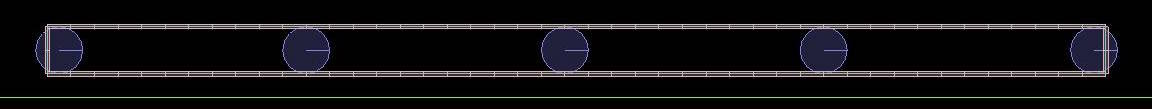
\includegraphics[width=0.8\textwidth]{conveyer} \\ \\}}
{\uncover<3->{\item The belt is construct by a linked chain of rectangular segments, and wrapping it around some wheels to function as a belt. The belt is moved by turning the wheels.}}
{\uncover<4->{\item When two objects contact each other, the friction between them tries to stop their surfaces from moving relative to each other.The belt friction coefficient is set high.}}
\end{enumerate}
\end{frame}
\begin{frame}{\centering{{\bf{Internal Circuitary Design}}}}
\begin{enumerate}
{\uncover<1->{\item \bf{Teleporter}}}
{\uncover<2->{\item
\centering 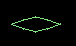
\includegraphics[width=0.3\textwidth]{teleporter} \\ \\}}
{\uncover<3->{\item This is a fictitious part of our project. We have used teleporter to move balls(fruits here) from one place to another. To implement this we overrided the b2ContactListener::BeginContact and EndContact functions.}}
{\uncover<4->{\item As soon a body touches the teleporter the mcontact bool variable becomes true and under step function of the base\_sim\_t class the code under the if condition runs and transforms the location of the body to another place.}}
\end{enumerate}
\end{frame}


\begin{frame}{\centering{{\bf{Internal Circuitary Design}}}}
\begin{enumerate}
{\uncover<1->{\item \bf{Balloons}}}
{\uncover<2->{\item
\centering 
\includegraphics[width=0.2\textwidth]{balloon} \\ \\}}
{\uncover<3->{\item We have used a balloon in the design. The balloon triggers the System of rotating flaps. The Balloon is a Box2D circle body, whose gravity has been scaled to a negative value.}}
\end{enumerate}
\end{frame}


\begin{frame}{\centering{{\bf{Internal Circuitary Design}}}}
\begin{enumerate}
{\uncover<1->{\item \bf{Five Gear Peeler}}}
{\uncover<2->{\item
\centering 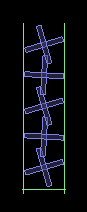
\includegraphics[width=0.2\textwidth]{5gear} \\ \\}}
{\uncover<3->{\item The peeler has 5 rotating gears that are set to same group index as not to collide with each other and are kinematic to rotate at same speed. They are fixed to that point by a joint to the base.}}

\end{enumerate}
\end{frame}

\begin{frame}{\centering{{\bf{Conclusions}}}}
\begin{enumerate}
{\uncover<1->{\item We saw how Box2D can be used to model physical systems on a computer, of which an example is our Rube-Goldberg machine simulation.}}
{\uncover<2->{\item Different aspects of the Box2D physics engine were demonstrated and a realistic simulation was carried out.}}
{\uncover<3->{\item Each segment of the machine is using a specific part of physics which emphasizes the importance of physics in designing machines.}}
\end{enumerate}
\end{frame}


\end{document}